

\tikzset{every picture/.style={line width=0.75pt}} %set default line width to 0.75pt        

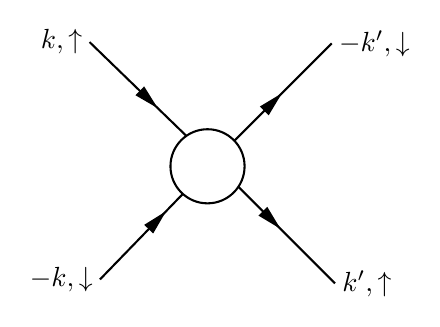
\begin{tikzpicture}[x=0.75pt,y=0.75pt,yscale=-1,xscale=1]
%uncomment if require: \path (0,300); %set diagram left start at 0, and has height of 300

%Straight Lines [id:da749548062064421] 
\draw    (97,121) -- (162.71,184.67) ;
\draw [shift={(129.85,152.84)}, rotate = 224.1] [fill={rgb, 255:red, 0; green, 0; blue, 0 }  ][line width=0.08]  [draw opacity=0] (12,-3) -- (0,0) -- (12,3) -- cycle    ;
%Straight Lines [id:da6891160905390028] 
\draw    (162.71,184.67) -- (215.3,237.27) ;
\draw [shift={(189,210.97)}, rotate = 225] [fill={rgb, 255:red, 0; green, 0; blue, 0 }  ][line width=0.08]  [draw opacity=0] (12,-3) -- (0,0) -- (12,3) -- cycle    ;
%Straight Lines [id:da7275939049575368] 
\draw    (102.03,235.38) -- (165.71,169.67) ;
\draw [shift={(133.87,202.53)}, rotate = 494.1] [fill={rgb, 255:red, 0; green, 0; blue, 0 }  ][line width=0.08]  [draw opacity=0] (12,-3) -- (0,0) -- (12,3) -- cycle    ;
%Straight Lines [id:da3845184529667176] 
\draw    (165.71,169.67) -- (213.71,121.67) ;
\draw [shift={(189.71,145.67)}, rotate = 495] [fill={rgb, 255:red, 0; green, 0; blue, 0 }  ][line width=0.08]  [draw opacity=0] (12,-3) -- (0,0) -- (12,3) -- cycle    ;
%Shape: Circle [id:dp7787521694372523] 
\draw  [fill={rgb, 255:red, 255; green, 255; blue, 255 }  ,fill opacity=1 ] (136,180.85) .. controls (136,170.99) and (143.99,163) .. (153.85,163) .. controls (163.71,163) and (171.71,170.99) .. (171.71,180.85) .. controls (171.71,190.71) and (163.71,198.71) .. (153.85,198.71) .. controls (143.99,198.71) and (136,190.71) .. (136,180.85) -- cycle ;

% Text Node
\draw (95,121) node [anchor=east] [inner sep=0.75pt]    {$\boldsymbol{k} ,\uparrow $};
% Text Node
\draw (100.03,235.38) node [anchor=east] [inner sep=0.75pt]    {$-\boldsymbol{k} ,\downarrow $};
% Text Node
\draw (217.3,237.27) node [anchor=west] [inner sep=0.75pt]    {$\boldsymbol{k} ',\uparrow $};
% Text Node
\draw (215.71,121.67) node [anchor=west] [inner sep=0.75pt]    {$-\boldsymbol{k} ',\downarrow $};


\end{tikzpicture}
